\documentclass[serif,onlymath,final,xcolor=table]{beamer}
%\documentclass[serif,mathserif,final]{beamer}
\mode<presentation>{\usetheme{Lankton}}
\usepackage{amsmath,url,graphicx,amssymb}
\usepackage{amsfonts}
\usepackage{ctable}
\usepackage{multirow}
\usepackage{algorithm}
\usepackage{algpseudocode}
\usepackage{pifont}
\usepackage{color}
\usepackage{subfigure}
\usepackage{enumitem}
\usepackage{sidecap}

\newcommand{\rom}[1]{\uppercase\expandafter{\romannumeral #1\relax}}

\newcommand{\todo}[1]{\textcolor{blue}{\bf #1}}
\newcommand{\fixme}[1]{\textcolor{red}{\bf #1}}

\newcommand{\mc}[3]{\multicolumn{#1}{#2}{#3}}
\newcommand{\mr}[2]{\multirow{#1}{0.10\textheight}{#2}}

\newcommand{\mylistbegin}{
  \begin{list}{$\bullet$}
   {
     \setlength{\itemsep}{-2pt}
     \setlength{\leftmargin}{1em}
     \setlength{\labelwidth}{1em}
     \setlength{\labelsep}{0.5em} } }
\newcommand{\mylistend}{
   \end{list}  }

\newcommand{\eg}{\textit{e.g.}}
\newcommand{\xeg}{\textit{E.g.}}
\newcommand{\ie}{\textit{i.e.}}
\newcommand{\etc}{\textit{etc}}
\newcommand{\etal}{\textit{et al.}}
\newcommand{\wrt}{\textit{w.r.t.~}}
\newcommand{\aka}{\textit{a.k.a.}}
\newcommand{\header}[1]{{\vspace{+1mm}\flushleft \textbf{#1}}}
\newcommand{\sheader}[1]{{\flushleft \textit{#1}}}
\newtheorem{thm:def}{Definition}

\newcommand{\floor}[1]{\lfloor #1 \rfloor}
\newcommand{\ceil}[1]{\lceil #1 \rceil}

\newcommand{\bx}{\boldsymbol{x}}
\newcommand{\by}{\boldsymbol{y}}
\newcommand{\ba}{\boldsymbol{a}}
\newcommand{\bw}{\boldsymbol{w}}
\newcommand{\bW}{\boldsymbol{W}}
\newcommand{\bfn}{\boldsymbol{f}}
\newcommand{\blambda}{\boldsymbol{\lambda}}
\newcommand{\btheta}{\boldsymbol{\theta}}

\newcommand{\cgg}{\textsc{CondGen}}
\newcommand{\mcW}{\mathcal{W}}
\newcommand{\mcT}{\mathcal{T}}
\newcommand{\mcY}{\mathcal{Y}}
\newcommand{\mcS}{\mathcal{S}}
\newcommand{\mcA}{\mathcal{A}}
\newcommand{\mcV}{\mathcal{V}}
\newcommand{\mcE}{\mathcal{E}}
\newcommand{\mcG}{\mathcal{G}}
\newcommand{\mcX}{\mathcal{X}}
\newcommand{\mcD}{\mathcal{D}}
\newcommand{\mcZ}{\mathcal{Z}}
\newcommand{\mcH}{\mathcal{H}}
\newcommand{\mcN}{\mathcal{N}}
\newcommand{\mcC}{\mathcal{C}}
\newcommand{\mcU}{\mathcal{U}}
\newcommand{\mcL}{\mathcal{L}}
\newcommand{\mcM}{\mathcal{M}}

\newcommand{\mbz}{\mathbf{z}}
\newcommand{\mbg}{\mathbf{g}}
\newcommand{\mbf}{\mathbf{f}}

\DeclareMathOperator*{\argmax}{arg\,max}
\DeclareMathOperator*{\argmin}{arg\,min}
\usepackage{amsmath,amsfonts,amssymb,pxfonts,eulervm,xspace}
\usepackage{graphicx}
\graphicspath{{./figures/}}
% \usepackage[orientation=landscape,size=custom,width=48,height=36,scale=.55,debug]{beamerposter}
\usepackage[orientation=portrait,size=a0,scale=1.4,debug]{beamerposter}
\usepackage{booktabs}
\usepackage{adjustbox}
\usepackage{multirow}
\newcommand\hmmax{0}
\newcommand\bmmax{0}
\usepackage{bbm}
\usepackage{dsfont}
\usepackage{mathtools}
\usepackage{amsmath,bm}
\usepackage{wrapfig}
\usepackage{enumerate}
% \usepackage{ragged2e}
% \justifying\let\raggedright\justifying

\newlength{\sepwidth}
\newlength{\colwidth}
\setlength{\sepwidth}{0.03\paperwidth}
\setlength{\colwidth}{0.45\paperwidth}

\newcommand{\separatorcolumn}{\begin{column}{\sepwidth}\end{column}}

\setbeamertemplate{bibliography item}{\insertbiblabel}
\setbeamertemplate{bibliography entry title}{}
\setbeamertemplate{bibliography entry location}{}
\setbeamertemplate{bibliography entry note}{}

\newcommand{\tabincell}[2]{\begin{tabular}{@{}#1@{}}#2\end{tabular}}  
\newcommand{\hide}[1]{} %hide

%-- Header and footer information ----------------------------------
\newcommand{\footleft}{}
\newcommand{\footright}{}
\newcommand{\ours}{BrainNNExplainer\xspace}
\newcommand{\back}{BrainNN\xspace}
% Color definition
\definecolor{sblue}{HTML}{02BCD4}
\definecolor{sred}{HTML}{F44436}
\definecolor{spink}{HTML}{E91E62}
\definecolor{sgreen}{HTML}{8BC34A}
\definecolor{spurple}{HTML}{3F51B5}
\definecolor{slightgreen}{HTML}{CCDE3A}
\definecolor{sorange}{HTML}{FE9800}
\definecolor{sgolden}{HTML}{FFC108}
\title{How Can Graph Neural Networks Help Document Retrieval: \\A Case Study on CORD19 with Concept Map Generation}
\author{Hejie Cui, Jiaying Lu, Yao Ge, Carl Yang \\(corresponding: j.carlyang@emory.edu)}
\institute{Department of Computer Science, Emory University, Atlanta, GA 30322, USA}
%-------------------------------------------------------------------


%-- Main Document --------------------------------------------------
\begin{document}
\begin{frame}
\begin{columns}[t]

% 	\begin{column}{2\colwidth+\sepwidth}
\begin{column}{0.97\linewidth}

\begin{block}{Contribution Highlights}
\begin{columns}	
\begin{column}{0.62\linewidth}
\begin{figure}[h]
\centering
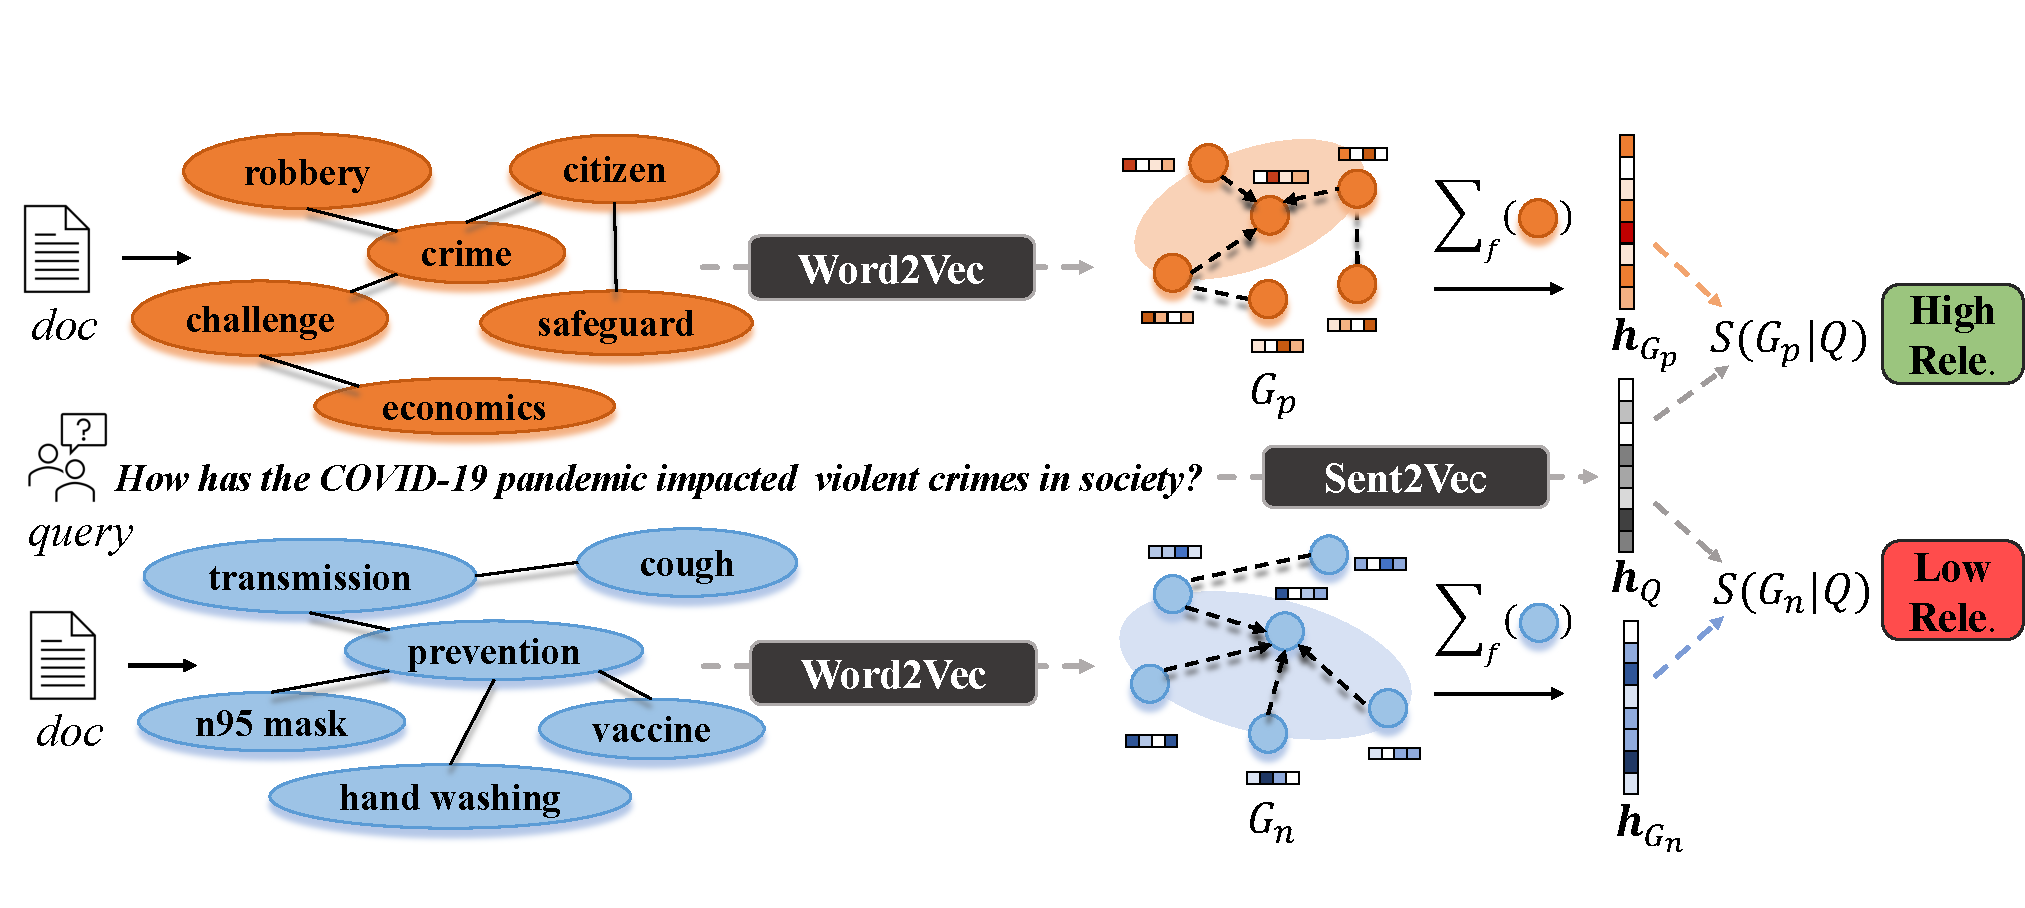
\includegraphics[width=0.8\textwidth]{figures/toy-example.pdf}
\caption{An overview of GNN-based document retrieval. }
\label{fig:model}
\end{figure}
\end{column}

\begin{column}{0.38\linewidth}
In this work, we explore how GNNs can help document retrieval with generated concept maps, consisting of:
\begin{list}{$\bullet$}{\leftmargin=1em \itemindent=0em}
\item Use constituency parsing to construct semantically rich concept maps from documents and design quality evaluation towards document retrieval.
\item Investigate two types of graph models for document retrieval: the \textit{structure-oriented} complex GNNs and our proposed \textit{semantics-oriented} graph functions.
\item Compare the retrieval results from different graph models and provide insights towards GNN model design for textual retrieval.
\end{list}
\end{column}

\end{columns}
\end{block}

\end{column}
\end{columns}

\begin{columns}[t]

%-- Column 1 ---------------------------------------------------
\begin{column}{0.31\linewidth}
% \vspace{-15pt}
%-- Block 1-1
\begin{block}{Introduction}
\textbf{Background}
\begin{list}{$\bullet$}{\leftmargin=1em \itemindent=0em}
\item Concept map models texts as a graph with words/phrases as vertices and relations between them as edges.
\item Empowered by the structured document representation of concept maps, it is intriguing to apply powerful GNNs for tasks like document classification and retrieval.
\end{list}

~\\
\textbf{GNNs for Document Retrieval}\\
Follow the common two-step practice for the large-scale document retrieval tasks: 
\begin{list}{$\bullet$}{\leftmargin=1em \itemindent=0em}
\item Step 1: initial retrieval on the whole corpus with full texts using BM25.
\item Step 2: re-rank with GNN models: construct concept map \(G = \{V, E\}\) for the top 100 candidate document and apply GNNs on each individual concept map, where node representation \(\bm{h}_i \in \mathbb{R}^{d}\) is updated through neighborhood transformation and aggregation. The graph-level embedding \(\bm{h}_G \in \mathbb{R}^{d}\) is summarized over all nodes with a read-out function. 
\item Given a triplet $(Q, G_p, G_n)$ composed by a relevant document $G_p$ and an irrelevant document $G_n$ to the query $Q$, the triplet loss function:
\begin{small}
\begin{align*}
L(Q, G_p, G_n)&=\max \{ S(G_n \mid Q) - S(G_p \mid Q)+\textit{margin}, 0\},
\end{align*}
\end{small}
where $S \left(G \mid Q \right)= \frac{\bm{h}_G \cdot \bm{h}_Q}{\|\bm{h}_G \|\|\bm{h}_Q\|}$, $\bm h_G$ is the learned graph representation and $\bm h_Q$ is the query representation from a pretrained model.
\item Retrieval in the testing phrase: documents are ranked according to the learned relevance score $S(G \mid Q)$.
\end{list}
\end{block}

%-- Block 1-2
\begin{block}{Concept Map Generation}
\begin{list}{$\bullet$}{\leftmargin=1em \itemindent=0em}
\item Concept map distill structured information hidden under unstructured text and represent it with a graph.
\item Existing methods based on name entity recognition (NER) or relation extraction (RE) suffer from limited nodes and sparse edges, rely on significant training data and predefined entities and relation types.
\item We propose to use POS-tagging and constituency parsing to increase node/edge coverage, thus bolstering the semantic richness of the generated concept maps for retrieval. The interactions among extracted nodes are constructed by sliding window. 
\end{list}
\end{block}


\end{column}

%-- Column 2 ---------------------------------------------------
\begin{column}{0.31\linewidth}
% \vspace{-15pt}
%-- Block 2-1

\begin{block}{GNN-based CP Representation}
\textbf{Type 1: Structure-oriented complex GNNs}
\begin{list}{$\bullet$}{\leftmargin=1em \itemindent=0em}
\item The discriminative power of structure-oriente complex GNNs stems from the 1-WL test for graph isomorphism.
\item We adopt two state-of-the-art ones, Graph isomorphism network (GIN) and Graph attention network (GAT).
\end{list}
~\\
\textbf{Type 2: Semantics-oriented permutation invariant graph functions}\\
In contrast, we propose a series of semantics-oriented graph functions: 
\begin{list}{$\bullet$}{\leftmargin=1em \itemindent=0em}
    \item \textit{N-Pool}: independently process each single node $v_i$ by multi-layer perceptions and then apply a read-out function to aggregate node embeddings $\bm a_{i}$ into the graph embedding $\bm h_{G}$, i.e., 
    \begin{small}
    \begin{equation*}
    \setlength{\abovedisplayskip}{3pt}
    \setlength{\belowdisplayskip}{3pt}
    \bm h_{G}=\operatorname{READOUT}\Big( \{\operatorname{MLP}(\bm a_{i}) \mid v_i \in V \}\Big).
    \end{equation*}
    \end{small}
    \item \textit{E-Pool}: the edge embedding of each edge $e_{ij}=(v_i, v_j)$ is obtained by concatenating the node embedding $\bm a_{i}$ and $\bm a_{j}$ on its two ends to encode first-order interactions, i.e., 
    \begin{small}
    % \begin{equation}
    \begin{align*}
    \setlength{\abovedisplayskip}{3pt}
    \setlength{\belowdisplayskip}{3pt}
    \bm h_{G}=\operatorname{READOUT}\Big(\left\{cat ( \operatorname{MLP}(\bm a_{i}), \operatorname{MLP}(\bm a_{j}) ) \mid e_{ij} \in E\right\}\Big).
    \end{align*}
    % \end{equation}
    \end{small}
    
    \item \textit{RW-Pool}: for each sampled random walk $p_i = (v_1, v_2, \ldots, v_m)$ that encode higher-order interactions among concepts, the embedding is computed by the sum of all node embeddings on it, i.e.,
    \begin{small} 
    % \begin{equation}
    \begin{align*}
    \setlength{\abovedisplayskip}{3pt}
    \setlength{\belowdisplayskip}{3pt}
    \bm h_{G}=\operatorname{READOUT}\Big( 
    \{ sum ( \operatorname{MLP}(\bm a_1), \operatorname{MLP}(\bm a_2), \\ \ldots, \operatorname{MLP}(\bm a_m) ) \mid p_i \in P \}\Big).
    \end{align*}
    % \end{equation}
    \end{small}
\end{list}
They preserve the \textit{message passing} mechanism of complex GNNs while focusing on the basic semantic units and different level of interactions between them.
\end{block}

\begin{block}{Experiment and Analysis (1/2)} 
\textbf{I. Evaluation of Concept Maps} 
\begin{table}[t]
\centering
\caption{The similarity of different concept map pairs.}
\resizebox{\textwidth}{!}{
\begin{tabular}{cccccc}
\toprule
Pair Type & \# Pairs & \bf NCR ($\%$)& \bf NCR+ ($\%$)& \bf ECR ($\%$) & \bf ECR+ ($\%$)\\ \midrule
Pos-Pos & 762,084  & 4.96 & 19.19 & 0.60 &  0.78       \\
Pos-Neg & 1,518,617 & 4.12 & 11.75 & 0.39 &  0.52       \\
\rowcolor{gray!20} (\textit{t-score}) & -  & (\textit{187.041}) & (\textit{487.078}) & (\textit{83.569}) &  (\textit{105.034})    \\
Pos-BM & 140,640 & 3.80 & 14.98 & 0.37 & 0.43 \\
\rowcolor{gray!20} (\textit{t-score}) & - & (\textit{126.977}) & (\textit{108.808}) & (\textit{35.870})  & (\textit{56.981}) \\
\bottomrule
\end{tabular}
}
\label{tab:structure}
\end{table}
$\rightarrow$ Concept maps can indicate query document relevance and provide additional discriminative signals based on the initial candidates. 
\end{block}
\end{column}


%-- Column 3 ---------------------------------------------------
\begin{column}{0.31\linewidth}

% \vspace{-15pt}     

\begin{block}{Experiment and Analysis (2/2)} 
\textbf{II. Retrieval Performance Results} 
\begin{table}[t]
\centering
% \small
\caption{\label{tab:perform}The retrieval performance of different models.}
\resizebox{\textwidth}{!}{
\begin{tabular}{cccccccc}
\toprule
\multirow{2.5}{*}{Type} & \multirow{2.5}{*}{Methods} & 
\multicolumn{2}{c}{\bf Precision ($\%$)}&\multicolumn{2}{c}{\bf Recall ($\%$)}&\multicolumn{2}{c}{\bf NDCG ($\%$)}\\
\cmidrule(lr){3-4} \cmidrule(lr){5-6} \cmidrule(lr){7-8} 
& & {\it k=$10$} & {\it k=$20$} & {\it k=$10$} & {\it k=$20$} & {\it k=$10$} & {\it k=$20$} \\
\midrule
\multirow{2}{*}{Traditional}
& BM25 & 55.20 & 49.00 & 1.36 & 2.39 & 51.37 & 45.91 \\
& Anserini & 54.00 & 49.60 & 1.22 & 2.25 & 47.09 & 43.82 \\
\midrule
\multirow{2}{*}{Structure-Oriented}
& GIN & 35.24 & 34.36 & 0.77 & 1.50 & 30.59 & 29.91 \\
& GAT & 46.48 & 43.26 & 1.08 & 2.00 & 42.24 & 39.49 \\
\midrule 
\multirow{3}{*}{Semantics-Oriented}
& \cellcolor{lightgray!20} N-Pool & \cellcolor{lightgray!20} 58.24 & \cellcolor{lightgray!20} 52.20 & \cellcolor{lightgray!20} 1.38 & \cellcolor{lightgray!20} 2.41 & \cellcolor{lightgray!20} 53.38 & \cellcolor{lightgray!20} 48.80 \\
& \cellcolor{lightgray!20} E-Pool & \cellcolor{lightgray!20} 59.60 & \cellcolor{lightgray!20} 53.88  & \cellcolor{lightgray!20} 1.40 & \cellcolor{lightgray!20} 2.49 & \cellcolor{lightgray!20} 56.11 & \cellcolor{lightgray!20} 51.16 \\
& \cellcolor{lightgray!20} RW-Pool &  \cellcolor{lightgray!20} \bf 59.84 & \cellcolor{lightgray!20} \bf 53.92 &  \cellcolor{lightgray!20} \bf 1.42 & \cellcolor{lightgray!20} \bf 2.53 & \cellcolor{lightgray!20} \bf 56.19 & \cellcolor{lightgray!20} \bf 51.41 \\
\bottomrule
\end{tabular}
}
\end{table}
~\\
\begin{list}{$\bullet$}{\leftmargin=1em \itemindent=0em}
\item Structural-oriented GNNs fail to improve the baselines (BM25, Anserini).
\item Semantics-oriented graph functions yield significant and consistent improvements over both baselines and structure-oriented GNNs.
\item Demonstrate the potential of designing semantics-oriented GNNs for textual reasoning tasks such as classification, retrieval, etc.
\end{list}
~\\
\textbf{III. Stability and Efficiency} 
   \begin{figure}
    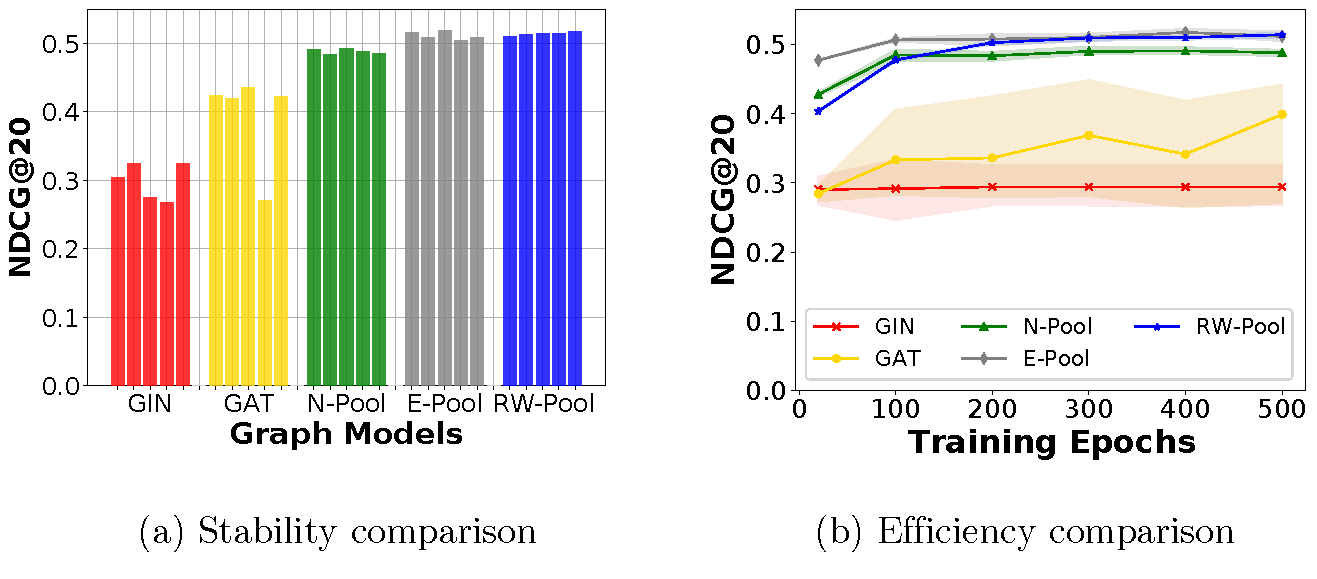
\includegraphics[width=\textwidth]{figures/stability_efficiency.pdf}
    \caption{Stability and efficiency comparison of different graph models.}
    \end{figure}
\begin{list}{$\bullet$}{\leftmargin=1em \itemindent=0em}
\item Semantics-oriented functions perform more stable and improve efficiently during training.
\item E-Pool and RW-Pool are consistently better than N-Pool, revealing the utility of simple graph structures.
\item RW-Pool converges slower but achieves better and more stable results in the end, indicating the potential advantage of higher-order interactions.
\end{list}
\end{block}
% \begin{block}{Conclusion Remarks}
% % \begin{enumerate}
% %     \item One
% %     \item Two
% %     \item Three
% % \end{enumerate}
% \end{block}

\begin{block}{Resources}
   \begin{figure}
    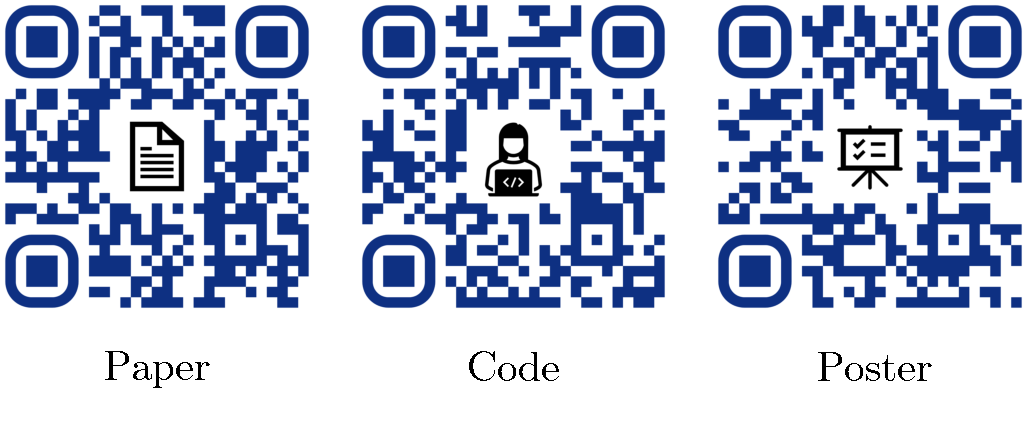
\includegraphics[width=\textwidth]{figures/resources.pdf}
    \end{figure}
\end{block}

\end{column}%3

\end{columns}

\end{frame}
\end{document}